This modulation can be encoded to retrieve the tag's data. The modulated back-scatter (or far-field coupling) retrieves the electromagnetic waves from the tag's antenna when not within the near-fields. These tags are typically designed for a frequency band such that there is a mismatch causing energy to be reflected back to the reader. The tag's impedance can be changed over-time to cause modulation, this modulation can be encoded by the reader to obtain the tag's data. Typically modulated back-scatter operates within the UHF frequency band. 

\begin{figure}[htp]
    \centering
    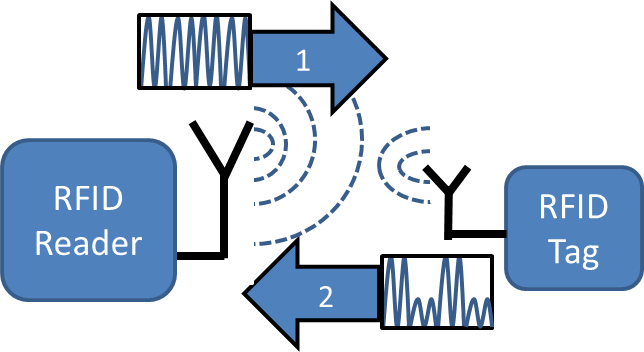
\includegraphics[scale=1.2]{Figs/FF_BS.png}
    \caption{Far-field power/communication set up RFID system. 1) RFID Reader transmits an emf 2) RFID Tag modulates and scatters the RFID Reader's emf 3) RFID Reader encodes the back-scatter signal from RFID Tag.}
    \label{fig:RFIDBlocks}
\end{figure}